\section*{Introduction}


\section*{Background}

Character-based phylogeny is a broad notion to represent an evolutionary history
describing the ancestral relationships among extant taxa or individuals. Recent applications show that
the model can be applied to study the evolution of mutations related to various genomic information, such as protein domains~\cite{Pr1} or markers in tumors.
Thus in  our formulation, it is not important whether we are actually studying taxa or
individuals or other genomic data.
We will follow the usual convention of calling
\emph{species} the units of study.
The main element of this notion is that the instance is also made of
a set of \emph{characters}, and each species is in a specific state for each character~\cite{Gusfield}.
The goal is to find a phylogeny where the known species are the leaves, and the
internal nodes are labeled---just as the leaves---by a state for each character.
For each edge $(x,y)$ of the phylogeny, the mutated characters along the edge are those whose
states are different in $x$ and $y$. The simplest case is when all characters are binary, that is only two states
($0$ and $1$) are possible,
modeling the situation  when each species has or not a given feature, such as
wings (a phenotypical trait) or the mutation encoding lactase persistence (a
genotypical trait).

Moreover, we are assuming a coalescent model, that is the fact that a characteristic
shared by a set of species can be traced back to a single ancestral species.
Assuming that the state $1$ encodes the fact that a species has a given
character (for example, the fact that the species has acquired a given mutation), the coalescent
model implies that the phylogeny is directed.
% and the label of the root is
% $\vec{0}$, and $(ii)$ for each character $c$ there is at most an edge $(x,y)$
% where $y$ is a child of $x$, and the state of $c$ in $x$ is $0$, but it is $1$
% in $y$.
Restrictions on the type of changes from zero to one and vice versa lead to a variety of specific models~\cite{felsenstein:inferring-phylogenies}.




The perfect phylogeny is one of the most investigated coalescent models~\cite{Gusfield}.
Conceptually the  model is based on the infinite sites assumption, that is no
character can mutate more than once in the whole tree.
The binary perfect phylogeny problem has received much attention, culminating
the linear time algorithm when all data is known~\cite{Gus91} and an efficient
algorithm when the input data is incomplete~\cite{Sha}.
While the infinite sites assumption is quite restrictive, the perfect phylogeny model
turned out to be splendidly coherent within the haplotyping problem~\cite{bo4,Gus02}, where we want to distinguish the two
haplotypes present in each individual when given only genotype data.
More precisely, the interest here is in computing a set of haplotypes and a perfect phylogeny such that the haplotypes
(i) label the vertices of the perfect phylogeny and (ii) explain the input set of genotypes.
This context has been deeply studied in the last decade, giving rise to a number of   algorithms~\cite{Boniz,Gus06}.
%
Still, the perfect phylogeny model and the assumptions that have been central in
the previous decades cannot be employed without adaptations or improvements.
A first generalization in the literature allows for more states
(but keeping the infinite sites assumption).
In the general case, the problem is NP-hard~\cite{BFW92}, but it has
an algorithm parameterized by the number of
states~\cite{DBLP:journals-siamcomp-Fernandez-BacaL03,kannan1997fast}.
The special cases when there are three or four possible states have more
efficient algorithms~\cite{dress1992convex,kannan1994inferring,gysel2012constructing}.


Even allowing more states cannot explain the biological complexity of
real data, when homoplasy events (such as recurrent mutations or back
mutations) are present.
Two cases where those limitations are evident are the study of carcinogenesis
and of protein domains.
Carcinogenesis consists of the factors
and mechanisms that cause the onset of cancer; it
results from many combinations of mutations, but only a few, called progression
pathways, seem to account for most human tumors~\cite{subramanian2012inference}.
The observation that tumors are evolving cell populations leads to phylogeny-based
studies. At the same time the intrinsic nature of quickly and degenerately
proliferating cancer cells, results in a relative high amount of sites with
multiple mutations (i.e., in violations of the infinite sites assumption).
A protein domain is
a part of protein sequence and structure that can evolve independently of the
rest of the protein chain. Many proteins consist of several structural
domains, while a domain may appear in a variety of different proteins. In this case
it is quite frequent to acquire a domain and then to lose it~\cite{przytycka2006graph}.

Thus a central goal of this paper  is to find a model that is more
widely applicable than the perfect phylogeny, while retaining  its computational
efficiency (in fact, more general models such as the Dollo and the Camin-Sokal
models are NP-hard~\cite{felsenstein:inferring-phylogenies}).
The problem of constructing  phylogenies where the deviations from perfect phylogeny are  small
has been tackled under the name of near perfect
phylogeny~\cite{DBLP:journals-siamcomp-Fernandez-BacaL03} or near perfect
phylogeny  haplotyping  problems~\cite{DBLP:conf-ismb-SatyaMAPB06}.
Especially the impossibility of losing a character that has been previously
acquired is too restrictive, resulting in more elaborated models,
such as the persistent character~\cite{Pr1} and the General Character
Compatibility~\cite{DBLP:conf-isbra-ManuchPG11,mavnuch2009generalised}.

More precisely, the  Persistent Perfect Phylogeny
model~\cite{DBLP:journals-tcs-BonizzoniBDT12} allows each character to be lost
(\ie{} going from state $1$ to $0$) in at most an edge of the phylogeny, while the
General Character Compatibility imposes some restrictions on the possible
mutations (that is on the possible states labeling the endpoints of an edge),
while allowing the input data to be a set of possible states for each character
of a species.

We present some new computational problems that can model the problem
of finding the smallest subset of input data that must be removed to
obtain a dataset that is compatible with a given topology.




\subsection*{The persistent perfect phylogeny}

Our approach follows~\cite{DBLP:journals-tcs-BonizzoniBDT12} to which we refer
the reader for a detailed discussion of PPP, while we give here
only a cursory treatment.
The input of the PPP problem is an  $n \times m$ binary matrix $M$ whose
columns are associated with the set $C  = \{c_1, \ldots,
c_m\}$ of characters and whose rows are associated with the set $S = \{s_1, \dots,
s_n\}$ of species.
Then $M[i,j] = 1$ if and
only if the species $s_i$ has character $c_j$, otherwise $M[i,j] = 0$.
The character $c$ is \emph{gained} in the only edge where its state goes from $0$ to
$1$ or, more formally, in the edge $(x,y)$ such that $y$ is a child of $x$ and
the $c$ has state $0$ in $x$ and state $1$ in $y$.
In this case the edge $(x,y)$ is labeled by $c^{+}$.
Conversely, $c$ is \emph{lost} in the edge $(x,y)$ if $y$ is a child of $x$ and
the $c$ has state $1$ in $x$ and state $0$ in $y$.
In the latter case the edge $(x,y)$ is labeled by $c^{-}$.
For each character $c$, we allow at most one edge labeled by $c^{-}$~\cite{zeng,DBLP:journals-tcs-BonizzoniBDT12}.
% \vspace{.1in}
% \noindent

\begin{definition}[Persistent Perfect Phylogeny]
\label{def:persistent-perfect-phylogeny}
Let $M$ be an  $n \times m$ binary matrix.
Then a \emph{persistent perfect phylogeny}, in short  \emph{ p-pp},
for $M$ is a rooted tree $T$ such that:
\begin{enumerate}
\item each node $x$ of $T$ is labeled by a vector $l_x$ of length $m$;
\item
  the root of $T$ is labeled by a vector of all zeroes,  while  for each  node
$x$ of $T$ the value $l_x[j]\in\{0, 1\}$
  represents the state of character $c_j$ in tree $T$;
\item
  each edge $e=(v,w)$ is labeled by at least a character;
\item
  for each character $c_j$ there are at most  two  edges $e=(x,y)$ and
$e'=(u,v)$
  such that $l_x[j] \neq l_y[j]$ and $l_u[j] \neq l_v[j]$
  (representing a change in the state of $c_j$).
In that case $e$, $e'$  occur along the same path
  from the root of $T$ to a leaf of $T$; if $e$ is closer to the root than $e'$,
  then $l_x[j]=l_v[j]=0$, $l_y[j]=l_u[j]=1$, and
  the  edge $e$ is labeled $c_j^{+}$,
  while  $e'$ is labeled $c_j^{-}$;
\item
  each row $r$ of $M$ labels exactly one node $x$ of $T$.
  Moreover the vector $l_{x}$ is equal to the row $r$.
\end{enumerate}
%Then we say that $T$ \emph{realizes} matrix $M$, that is $M$ admits a p-pp tree.
%Whenever  a binary matrix $M$ admits a p-pp tree we say  that $M$ is \emph{solvable}.
\end{definition}

Let $s$ be a species and let $c$ be a character such that, in a persistent
perfect phylogeny $T$, the path from the root of $T$ to $s$ traverses an edge
labeled $c^{-}$.
Then $c$ is called persistent for $s$ in $T$.

The Persistent Perfect Phylogeny problem asks to find, if it exists, a
persistent perfect phylogeny for a given binary matrix $M$.
We can restate the PPP  problem  as a
variant  of the Incomplete Directed Perfect Phylogeny~\cite{Sha} by transforming
the complete input matrix into an incomplete matrix, called extended matrix.

\begin{definition}[Extended Matrix]
\label{def:Extended-Matrix}
Let $M$ be an instance of the PPP problem. The \emph{extended matrix}
associated with $M$ is an ${n \times 2m}$ matrix \me  over alphabet $\{0,1,?\}$
which is obtained by replacing each column $c$ of $M$ by a pair of columns
$(c^{+}, c^{-})$, where $?$ means that the value of such cell is not given.
Moreover for each   row $s$  of $M$
% \begin{enumerate}
% \item
if $M[s,c] = 1$, then  $M_e[s,c^{+}] = 1$ and $M_e[s,c^{-}] = 0$,
% \item
while if $M[s,c] = 0$, then  $M_e[s,c^{+}] = ?$ and $M_e[s,c^{-}] = ?$.
% ,
% otherwise $M_e[s,c^{+}] =0$ and $M_e[s,c^{-}] = 0$.
% \end{enumerate}
\end{definition}

% \begin{figure}[htbp]
% %\subfigure[A binary  matrix $M$ and the extended matrix of size $n \times 2m$]
% \begin{center}
% \includegraphics[width=0.90\textwidth]{M_Me}
% \end{center}
% \caption{A binary  matrix $M$ and the extended matrix of size $n \times 2m$}
% \label{fig:standard-tree2}
% \end{figure}


In this case the characters $(c^{+}, c^{-})$ are called conjugate.
Informally, the assignment of the \emph{conjugate} pair $(?,?)$ in a species
row $s$ for two conjugate characters ($c^{+}, c^{-}$) means that
character $c$ could be persistent in species $s$, \ie it is first gained and
then lost.
On the contrary, the pair $(1,0)$ means that character $c$ is only gained by
the species $s$.
% Finally, the pair $(0,0)$ means that character $c$ is never  gained  by
% the species $s$.
A \emph{completion}  of  a pair $(?,?)$  associated to a species $s$ and
characters ($c^{+}, c^{-}$) of  \me  consists
of forcing $\me [c^{+},s]=\me [c^{-},s]=0$ or  $\me [c^{+},s]=\me [c^{-},s]=1$,
while a partial \emph{completion}  \me is a completion of some of its conjugate
pairs.
% A completion is \emph{full} if all its conjugate pairs are completed.
Notice that $M$ admits a persistent phylogeny  if
and only if there exists a completion  of $M_e$ admitting a directed perfect
phylogeny~\cite{DBLP:journals-tcs-BonizzoniBDT12}.


 %\begin{comment}


%\end{comment}

A fundamental contribution of~\cite{DBLP:journals-tcs-BonizzoniBDT12}, building
upon~\cite{Sha}, is to frame the problem as a graph theory question.
We briefly recall here the two graphs that are used in the description of the algorithm.


Let $M$ be a binary matrix and let $c_{1}$, $c_{2}$ be two characters of $M$.
Then the configurations induced by the pair $( c_{1}, c_{2} )$ in $M$ is the
set of ordered pairs $( M[s,c_{1}], M[s,c_{2}])$ over all species $S$.
Two characters $c_{1}$ and $c_{2}$ of $M$ are \emph{conflicting} if and only if
the configurations induced by such pair
of columns is the set of all possible pairs $( 0,1)$, $( 1,1) $, $(1,0) $ and
$( 0,0) $.
The \emph{conflict graph}  $G_c =( C,E_{c}\subseteq C \times C)$ of a matrix $M$
has vertices $C$ and as edges the pairs $(c_{i}, c_{j})$ of conflicting characters (see Figure~\ref{fig:standard-tree}).
%
We also need some graph-theoretic definitions.
A graph without edges is called \emph{edgeless}.
A connected component is called \emph{nontrivial} if it has more than one
vertex.


%\begin{figure}[htbp]
%\begin{center}
%\includegraphics[width=0.50\textwidth]{m_Gc_p-pp_colored}
%\end{center}

%\caption{A matrix and its conflict graph}
%\label{fig:standard-tree}
%\end{figure}




The second graph used in the algorithm provides a representation of a  completion of characters of an extended matrix.
The \emph{red-black graph} $\grb=\langle V,E \rangle$  associated to an extended matrix \me
is the edge-colored graph where (i)
the vertices are the species and the conjugate pairs of \me (that is
for each two conjugate
characters $c^{+}$ and $c^{-}$, only $c$ is a vertex of \grb), (ii) a pair $(s,c)$
is a black edge iff the conjugate pairs
$c^{+}$ and $c^{-}$ are still incomplete in matrix \me and
$M_e[s,c^{+}]=1$ and
$M_e[s,c^{-}]=0$, (iii)
$(s,c)$ is a red edge iff the conjugate pairs
$c^{+}$ and $c^{-}$ are completed as $M_e[s,c^{+}]=M_e[s,c^{-}]=1$.


\section*{Results and discussion}


\subsection*{Species-Driven Phylogeny}

It is a well-known fact that matrices admitting a galled tree are a
subset of those admitting a persistent phylogeny~\cite{gusfield_optimal_2004}.
In this section we will present the notion of species-driven phylogeny
and we will show that the set of  matrices admitting a galled tree is
properly contained in the set of matrices admitting a species-driven phylogeny.


\begin{definition}
\label{definition:species-driven}
Let $T$ be a persistent phylogeny.
Then $T$ is called \emph{species-driven} if there exists an ordering
$(s_{1}, \ldots , s_{n})$ of all species of $T$ such that for edge $e_{j}$
labeled by a negated character $c_{j}^{-}$  and lying on the path from
the species $s_{i}$ to the root of $T$, there is a species $s_{h}$
with $h < i$ such that the path from $s_{h}$ to the root of $T$
traverse the edge labeled $c_{j}^{+}$.
\end{definition}

In the species-driver persistent perfect phylogeny the basic idea is that, given  a binary matrix, we ask to build a tree  $T$ and an ordering of species  of the input matrix, such that if a character is lost by a species $s_i$ in the ordering, the (positive) character must be along the path from the root to a species $s_j$ such that $j < i$, i.e. $s_j$ occurs before $s_i$ in the ordering.

The exponential-time algorithms for persistent
phylogeny~\cite{DBLP:journals-tcs-BonizzoniBDT12,bonizzoni_explaining_2014}
can be applied also for this problem, by providing a procedure to test
if a given solution is also a species-driven.

In fact, those algorithm are based on computing all possible sequences
of characters corresponding to a visit of the tree $T$.
The more efficient algorithm of~\cite{bonizzoni_explaining_2014} is
able to speed up the computation when the conflict graph has no edge:
in this case the solution consists of computing the perfect phylogeny
on some submatrices.
Since the perfect phylogeny of a matrix is unique, this strategy does
not skip any possible species-driven phylogeny.

But Definition~\ref{definition:species-driven} suggest a test that is
very expensive to compute, since it requires (in the worst case) to
compute all possible permutations of the species.
By provide now an alternative definition: in the following we will
prove that those two definitions are equivalent.


\begin{definition}
\label{definition:species-driven-2}
Let $T$ be a persistent phylogeny.
Then $T$ is called \emph{species-driven} if there exists a permutation
$(d_{1}, \ldots , d_{k})$ of all characters that are negated in $T$
such that for each $d_{i}$ there is a species $x_{i}$ whose path from
the root of $T$ to $x_{i}$ traverses the edge $d_{i}^{+}$ but does not
traverse any edge $d_{j}^{-}$ with $j \le i$.
\end{definition}

\begin{lemma}
\label{lemma:equivalent-species-driven}
Definitions~\ref{definition:species-driven}
and~\ref{definition:species-driven-2} are equivalent.
\end{lemma}

\begin{proof}
TODO
\end{proof}

The importance of Definition~\ref{definition:species-driven-2} is that
a much simpler test to determine if a solution computed by the
algorithm of~\cite{bonizzoni_explaining_2014} is actually a
species-driven phylogeny.

\begin{lemma}
\label{lemma:same-order-of-algorithm-for-species-driven-test}
Let $T$ be a species-driven phylogeny and let $(d_{1}, \ldots,
d_{k})$ be the permutation of all characters that are negated in $T$
that satisfies Definition~\ref{definition:species-driven-2}.
Then there exists a visit of $T$ that traverses in order the edges
labeled by $d_{1}^{-}, \ldots, d_{k}^{-}$.
\end{lemma}

\begin{proof}
TODO
\end{proof}

\subsection*{Minimum Column Removal}

A simple formulation of our problem assumes that we have in input a
topology $T$ with $n$ leaves and a matrix $M$ with $n$ rows.
In this case we already know that the species of $M$ labels the leaves
of $T$.
The only allowed modification to the matrix $M$ is to remove some columns.
We have three different formulation of the problem according to the
fact that we want a perfect phylogeny, a persistent phylogeny or a
species-driven phylogeny.


In this paper we will consider only trees where the leaves are labeled
by the species, and no other node is labeled.
We will also allow only one character to label each edge of the tree.





The problem of removing some columns so that the remaining columns
have a perfect phylogeny has been widely studied in the
literature~\cite{rens_snv-ppilp:_2015} and is is usually  modeled as
finding an independent set of the conflict graph.
This approach relies on the fundamental characterization of matrices
that admit a perfect phylogeny as the matrices satisfying the 4-gamete test.
On one hand, reducing to an NP-hard problem does not lead to a
polynomial-time algorithm, but several exponential-time but practical
algorithms for independent set are known.

\begin{definition}
\label{definition:perfect-problem}
Given a $n\times m$ matrix $M$ and a tree $T$ with $n$ leaves and $e$
edges, the
\emph{Minimum Column Removal Fixed-Topology Perfect Phylogeny} (Min
C-Perf) problem asks for a set $X$ of $e$ columns of $M$ such
that removing $X$ from $M$ results in a matrix that is realized by a
perfect phylogeny on $T$.
\end{definition}


The Min C-Perf problem is NP-hard~\cite{karp_reducibility_1972}.
We sketch here a reduction from Min Independent Set on cubic graphs,
which is already known to be APX-hard~\cite{alimonti_apx-completeness_2000}.
Let $G=(V,E)$ be a cubic graph.
Then $M$ is a matrix that has a row made entirely of zeroes, and for
each arc $(v_{i}, v_{j})$ of $G$ there are three rows $r_{i,j,01}$,
$r_{i,j,10}$, $r_{i,j,11}$, where  $r_{i,j,01}$ is made of zeroes,
except for character $c_{j}$,
$r_{i,j,10}$  is made of zeroes,
except for character $c_{i}$, and $r_{i,j,11}$  is made of zeroes,
except for characters $c_{i}$ and $c_{j}$.
The resulting matrix has $|V|$ characters and $3|V|+1$ rows.
It is immediate to notice that each pair of characters $(c_{i},
c_{j})$ are conflicting, while no other pairs of characters are conflicting.
Each column of $M$ contains exactly $4$ ones, therefore let $T$ be a tree
consisting of a root and $k$ $P_{5}$s (paths consisting of $5$
vertices and $4$ edges) all starting from the root of $T$.
It is immediate to prove that if $G$ has an independent set of size
$k$, then $T$ realizes a submatrix of $M$ with $k$ columns.



\begin{definition}
\label{definition:persistent-problem}
Given a $n\times m$ matrix $M$ and a tree $T$ with $n$ leaves and $e$
edges, the
\emph{Minimum Column Removal Fixed-Topology Persistent Phylogeny} (Min
C-Pers) problem asks for a smallest set $X$ columns of $M$ such
that removing $X$ from $M$ results in a matrix that is realized by a
persistent phylogeny on $T$.
\end{definition}

Notice that the Min C-Pers problem inherits the NP-hardness of Min
C-Perf, but it is defined as an actual optimization
problem~\cite{ausiello_approximate_1995}, while the Min C-Perf problem
is a decision problem~\cite{garey_computer_1979}.
In fact, it is not possible to define  Min C-Perf as an optimization
problem, since the number of columns to keep is equal to the number of
edges of $T$.

\begin{definition}
\label{definition:species-driven-problem}
Given a $n\times m$ matrix $M$ and a tree $T$ with $n$ leaves and $e$
edges, the
\emph{Minimum Column Removal Fixed-Topology Species-Driven Phylogeny} (Min
C-SD) problem asks for a smallest set $X$ columns of $M$ such
that removing $X$ from $M$ results in a matrix that is realized by a
species-driven persistent phylogeny on $T$.
\end{definition}


In the case of persistent phylogeny this approach cannot be used since there is no induced submatrix.

Now, a complex red-black graph is characterized by the fact that it induces a
conflict-graph with more than one non trivial component as proved in
Lemma~\ref{lem:twoComp}.

More precisely,  we show that every successful
reduction of  $G_{RB}$ starts with the realization of a set of
characters with special properties and tree $T$ has also a special structure.
In fact, each tree $T$ consists of  $k \geq 2$ subtrees $T_1, \cdots, T_k$
such that there exists a unique path, called \emph{split path}, from root $r$
of $T$ to a node $x$ (called the \emph{end} of the split path)
that is  the root of all  trees $T_1, \cdots, T_k$.
The set of characters labeling a split path is called a {\em split set} for
$G_{RB}$.
Notice that the split set contains only positive characters (otherwise we would
have a null
character in $\grb$) that are negated in some edge of $T$ (otherwise we would
have a universal character).
\begin{comment}
Then the realization of $C'$ divides the red-black graph into $k$ distinct
components each representing a subtree $T_i$ of tree $T$.  Moreover,  after the
realization of set
$C'$  in the red-black graph,  the   conflict-graph induced by the new
red-black graph  has no
conflicting-pair including characters of $C'$ ($C'$ is a {\em conflict-free
  split set}).
\end{comment}

Our main characterization of complex red-black graphs follows.

\begin{lemma}
  \label{lem:twoComp}
Let $M_e$ be an extended matrix whose red-black graph  $G_{RB}$
is connected, complex and solved by a standard tree $T$.
Then $G_{c}$ has  at least two non trivial
connected components.
\begin{comment}
 $G_{c_1} \cdots G_{c_k}$ with $k \geq 2$.
and the tree $T$
consists of a unique path from the root to a node $x$ such that the label
sequence for node $x$ split the red-black graph into at least two disjoint
red-black graphs.
\end{comment}
\end{lemma}


\begin{proof} % (of Lemma~\ref{lem:twoComp})
Since \grb is connected, there is a split path ending in a node $x$. and let
$X$ be the corresponding split set.
We already know that each character in
$X$ must be negated in $T$.

Let $T_{1}$ be a generic subtree of $T$ and let $S_{1}$ be its set of species.
First we notice that if a character $c^{+}$ appears in $T_{1}$, then
$\me[c^{+},s]=\me[c^{-},s]=0$ for each species $s$ in any other subtree of $T$.
Consider now the case where the character $c^{+}$ appears in $X$ and $c^{-}$
appears in $T_{1}$; in this case $\me[c^{+},s]=1$, $\me[c^{-},s]=0$ for each
species $s$ in any other subtree of $T$.
By the generality of $T_{1}$, all characters that change state in one of the
other subtrees cannot change state in $T_{1}$.
This fact make impossible to have two conflicting characters labeling edges of
two different subtrees, hence no connected component of $G_{c}$ spans characters
appearing in two different subtrees.

Now we are going to prove that there are at least two nontrivial connected
components of $G_{c}$.
Assume to the contrary that that $T$ is a counterexample with the minimum number
of negated characters.
Notice now that each subtree has at least an edge labeled by a negated
character, for otherwise there would be a species that can be realized,
contradicting the hypothesis that \grb is complex
Since there are at least two subtrees $T_{1}$ and $T_{2}$, w.l.o.g. we can
assume that $c_{1}^{-}$ appears in $T_{1}$ and $c_{2}^{-}$ appears in $T_{2}$.
By minimality of the number of negated characters and the first part of the
proof, both $c_{1}$ and $c_{2}$ are involved in two different conflicts that are
edges of two different connected components of $G_{c}$.
Since both components have an edge, they are nontrivial.
\end{proof}




\subsection*{A characterization of matrices without a pp tree solution}


Now, given
an incomplete extended matrix $M_e$ associated to a red-black graph,  the
matrix $Grid$  has an entry $ [e, ij]$ for each edge $e= (x,y)$ of the
conflict-graph  and configuration $ij$  for the characters $x$ and $y$ of edge
$e$. Then entry $Grid[e, ij]$ reports the chains of species (rows of matrix
$M_e$)  in poset $(P,<_s)$ that induce the configuration $ij$ for edge $e$.
Then a \initial positive path-sequence is identified by merging entries (i.e
chains) of the grid-matrix $Grid[e, ij]$.  In fact, observe that  the  entry of
$Grid[e, ij]$ consists of  species that once they are solved in the red-black
graph, i.e. they become isolated nodes in the red-black graph. Consequently,
the rows corresponding to  the configuration $ij$
they induce in the original matrix $M$, are  removed from $M$. It follows that
the edge $e$ is not present in the  conflict-graph induced in $M$ by the rows
and columns
that are in the connected red-black graph (see Definition
\ref{def:conflict-induced-by-red-black}).


Let  $Grid$ be the grid of a conflict graph $G_{c}$ and  let $e=(x,y)$ be an
edge of $G_{c}$.
Let $Good(e)$  be  the union of all species that are in the entries
$Grid[e,ij]$ for $ij \in \{10,01,00\} $.
\begin{lemma}\label{lem-inters-vuota}
  Assume that the conflict  graph  $G_c$   for the binary matrix $M$ is formed
by only one non trivial connected component and the red-black graph $G_{RB}$
for $M$ is connected. Assume that
  $\bigcap_{e \in E(G_c)} Good(e) = \emptyset$.
  Then $M$ does not admit a persistent perfect phylogeny.
\end{lemma}
\begin{proof}
  First let us assume that all universal characters have been realized in the
red-black graph $G_{RB}$, thus the matrix $M$ has no universal character.

  By applying Lemma~\ref{lem:twoComp}, it must be that the conflict graph
consists
  of at least two non trivial connected components, thus obtaining a
contradiction.


\end{proof}



By Lemma~\ref{lem-inters-vuota} we can show that exists a infinite set of
matrix that do not admit a p-pp tree. These matrices have associated a
connected conflict graph that is an unchordal cycle and $\bigcap_{e \in E(G_c)}
Good(e) = \emptyset$.


\begin{theorem}
  \label{teo_esistenza_PM}
  For each $n \ge 4$ exists a $n \times n$ forbidden matrix which does not
admit persistent perfect phylogeny and such
  that it does not contain a smaller forbidden matrix.
  % Exists an infinite set $P_M$ of $n \times n$ forbidden distinct matrix, with $n \ge 4$, wherdove per matrici distinte si intende che $\forall M, M' \in P_M$, $M$ non è una sotto-matrice indotta da $M'$ e viceversa, che non ammettono filogenesi perfetta persistente.
\end{theorem}
\begin{proof}
  For each $n\ge 4$, $\exists$ a $n \times n$ binary matrix $M$, such that
$\forall$ $1 \le i < n$ the species at the row $i$ has the pair of characters
$(c_i, c_{i+1})$ and the species at the row $n$ has the pair $(c_1, c_n)$.

  By construction $M$ has associated an unchordal cycle conflict graph $G_c$
and such that $\bigcap_{e \in E(G_c)} Good(e) = \emptyset$. Consequently by the
Lemma~\ref{lem-inters-vuota} the matrix $M$ does not admit persistent perfect
phylogeny.

\end{proof}




\subsection*{Examples}

The following matrix $\mathcal M$ admits a pp tree but has no path-sequence.

\begin{table}
\centering
\begin{tabular}{c|cccccccccccccccc}
    $s/c$ & $c_1$ & $c_2$ & $c_3$ & $c_4$ & $c_5$ & $c_6$ & $c_7$ & $c_8$ & $c_9$ & $c_{10}$ &
$c_{11}$ & $c_{12}$ & $c_{13}$ & $c_{14}$ & $c_{15}$ & $c_{16}$\\\hline
1 & 1 & 1 & 1 & 0 & 0 & 0 & 1 & 0 & 1 & 0 & 0 & 0 & 0 & 0 & 0 & 0 \\
2 & 1 & 1 & 1 & 0 & 0 & 0 & 1 & 1 & 0 & 1 & 0 & 0 & 0 & 0 & 0 & 0 \\
3 & 1 & 1 & 0 & 1 & 0 & 0 & 1 & 1 & 0 & 0 & 1 & 0 & 0 & 0 & 0 & 0 \\
4 & 1 & 1 & 0 & 1 & 0 & 0 & 0 & 1 & 0 & 0 & 0 & 1 & 0 & 0 & 0 & 0 \\
5 & 1 & 0 & 1 & 1 & 1 & 0 & 0 & 0 & 0 & 0 & 0 & 0 & 1 & 0 & 0 & 0 \\
6 & 1 & 0 & 1 & 1 & 1 & 1 & 0 & 0 & 0 & 0 & 0 & 0 & 0 & 1 & 0 & 0 \\
7 & 0 & 1 & 1 & 1 & 1 & 1 & 0 & 0 & 0 & 0 & 0 & 0 & 0 & 0 & 1 & 0 \\
8 & 0 & 1 & 1 & 1 & 0 & 1 & 0 & 0 & 0 & 0 & 0 & 0 & 0 & 0 & 0 & 1 \\
\end{tabular}
\caption{A binary matrix  $\mathcal M$ on $8$ species and $16$
  characters that has a persistent phylogeny, but no species-driven phylogeny}
\label{table:matAmmetteP-pp}
\end{table}


\begin{figure}[htbp]
\centering
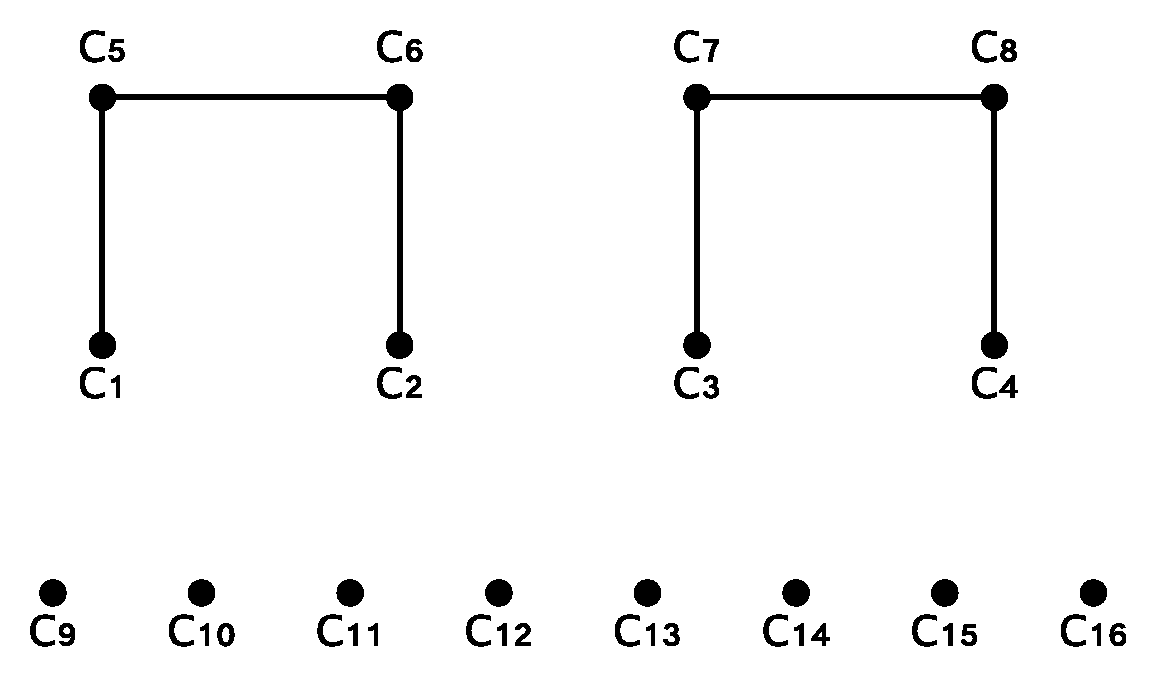
\includegraphics[height=10cm, width=8cm,keepaspectratio]{GrafoConflitti1}
\caption{Conflict graph associated to the matrix  $M$ given in Fig.~\ref{table:matAmmetteP-pp} }
\label{fig:GcM}
\end{figure}


Figure~\ref{fig:GcM} illustrates the conflict graph of matrix $M$. It consists
of two non trivial connected components and singletons.

It is immediate to verify that the red-black graph for matrix $M$ does not have
a species $s$ that can be realized, as  $\bigcap_{e \in E(G_c)}Good(e) =
\emptyset$.
Moreover observe that all species are not comparable under the $<_s$-relation.
The red-black graph  for $M$   admits a successful reduction   $r $ given by
the sequence $\langle c_1, c_2, c_3, c_4, c_5, c_6, c_7, c_8, c_{13}, c_{14},
c_{15}, c_{16}, c_9, c_{10}, c_{11}, c_{12} \rangle$.
The persistent phylogeny for matrix $M$ is given in Figure ~\ref{fig:albero1}.



A similar problem can be defined when we also have a topology T in input.

Special case: the input matrix has a perfect phylogeny on T and we want a persistent phylogeny. In that case a matching on the conflict graph suffices.

Also maximization version, where we want to maximize the number of columns that are kept.

Notice that allowing only the removal of some rows does not really make sense if only leaves of T can be labeled by some species.

\subsection{Minimum Matrix Editing}

The problem asks for changing the fewest possible matrix entries, so that the resulting matrix has a (perfect/persistent/species-driven) phylogeny. 

\subsection{Minimum Matrix Removal}

The problem asks for deleting the fewest possible rows/columns, so that the resulting matrix has a (perfect/persistent/species-driven) phylogeny.

\section{Conclusions}

We have presented some new computational problems that model\cite{bonizzoni_when_2014}



%%% Local Variables:
%%% mode: latex
%%% TeX-PDF-mode: t
%%% TeX-master: "fixed-topology-ppp.tex"
%%% buffer-file-coding-system: utf-8
%%% End:
